%=========================================================================
% (c) 2014, 2015 Josef Lusticky

\section{Hardware and cabling}\label{sec:setup-hardware}
Figure~\ref{fig:setup-supermicro-board} shows the block diagram of the Supermicro motherboard.
The Intel Xeon E5-2630 v2 processor was plugged into the front CPU socket 00.
To plug the Mellanox ConnectX-3 EN adpater into the PCIE 3.0 x16 slot,
a proprietary Supermicro riser card needed to be used.
The Mellanox ConnectX-3 EN card was then plugged into this riser card.
The front CPU is directly connected to the PCI-Express links, so no QPI links were used in the experiments.
\begin{figure}
	\centering
	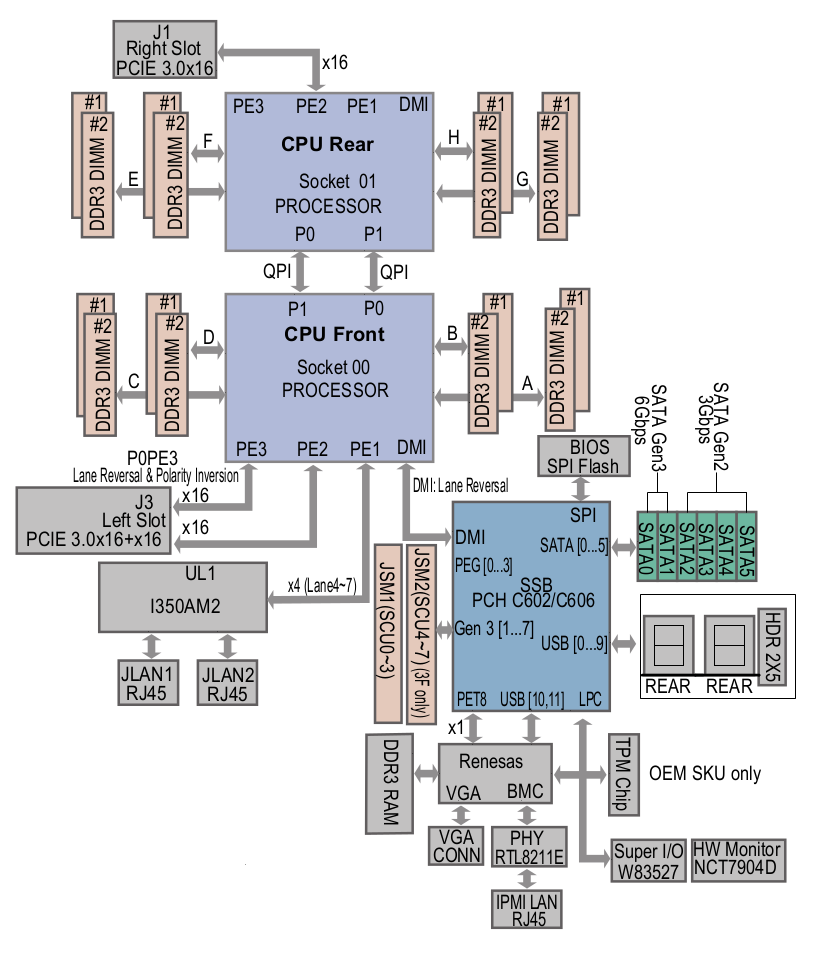
\includegraphics[width=14.5cm,keepaspectratio]{fig/supermicro-board.png}
	\caption{Supermicro motherboard's block diagram}
	\label{fig:setup-supermicro-board}
\end{figure}

The server was put to the same rack as the Spirent hardware generator.
A pair of 40GBASE-SR4 multimode fiber cables with QSPF connectors
was used to connect Spirent with the Mellanox ConnectX-3 EN adapter.
